\documentclass{ximera}
\usepackage{OERLinearAlgebra}


\usepackage{mathtools}
\usepackage{tikz-3dplot}

\author{Anna Davis \and Rosemarie Emanuele} \title{Parametric Equations of Lines} \license{CC-BY 4.0}

\begin{document}

\begin{abstract}
  We use parametric equations to represent lines in $\RR^2$ and $\RR^3$.
\end{abstract}
\maketitle

At this point you should be very familiar with graphing linear equations of the form $y=mx+b$, where $m$ is the slope of the line and $b$ is the $y$-intercept.  Unfortunately, there is no equivalent way of representing lines in $\RR^3$, or better yet, $\RR^n$.  In this module we will develop an alternative way of representing lines.

\section*{Parametric Lines in $\RR^2$}
\begin{initprob}\label{init:paramline2d}
Imagine a ladybug crawling around a plane.  At every instant in time, the ladybug's position in the plane can be described by an ordered pair $(x, y)$.  Coordinates $x$ and $y$ are functions of time.  Suppose the position of the ladybug at time $t$ is given by:
\begin{align*}
x&=2t-1\\
y&=-3t+6
\end{align*}
Our goal is to sketch the path of the ladybug during the time interval $0\leq t\leq 3$.  To do this we will make a table of values, just like you did when you first started sketching graphs of functions.
$$\begin{array}{|c|c|c|}  
 \hline t& x & y\\ 
 \hline 0 & -1 & 6\\ 
 \hline 1 & 1 & 3 \\
 \hline 2 & 3& 0\\
 \hline 3 & 5& -3\\
 \hline
 \end{array}$$
 
The point $(x, y)$, corresponding to each value of $t$ is the location of the ladybug in the coordinate plane at time $t$. 
 \begin{image}[2.5in]
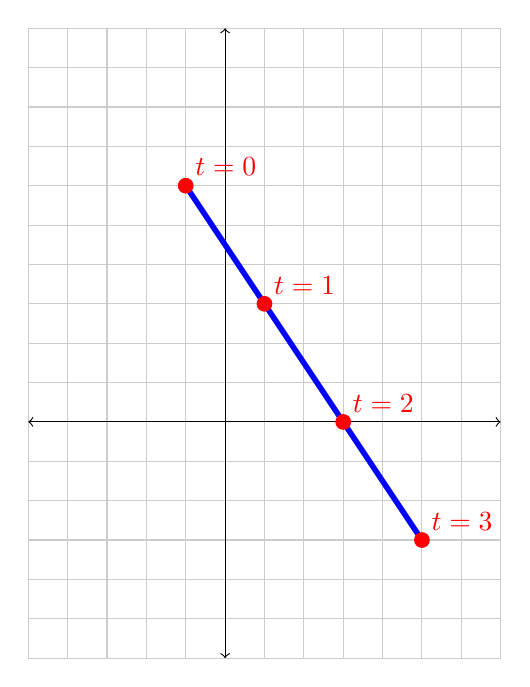
\begin{tikzpicture}[scale=0.5]
\draw[thin,gray!40] (-5,-6) grid (7,10);
  \draw[<->] (-5,0)--(7,0);
  \draw[<->] (0,-6)--(0,10);
  
\draw[line width=2pt,blue](-1,6)--(5,-3) ;

\fill[red] (-1,6) node[above right]{$t=0$} circle (0.2cm);
\fill[red] (1,3) node[above right]{$t=1$} circle (0.2cm);
\fill[red] (3,0) node[above right]{$t=2$} circle (0.2cm);
\fill[red] (5,-3) node[above right]{$t=3$} circle (0.2cm);
 
\end{tikzpicture}
\end{image}

It appears that the points corresponding to $t=0, 1, 2, 3$ lie on a line with slope $-\frac{3}{2}$.  In the next problem we will find the equation of the line that contains the path of the ladybug.
\end{initprob}

\begin{initprob}\label{init:paramline2dpart2}
In Exploration Problem \ref{init:paramline2d} we considered equations
\begin{align*}
x&=2t-1\\
y&=-3t+6
\end{align*}
that described the path of a ladybug in the plane.  We will now consider these equations in a broader context as simply describing a curve in the plane.  We conjectured that the curve described by these equations is a line with slope $-\frac{3}{2}$.  We will now find the equation of this line.

One approach to finding the equation is to solve one of the given equations for $t$, then substitute into the other equation.
Solving $x=2t-1$ for $t$ gives us
$$t=\frac{1}{2}x+\frac{1}{2}$$
Substituting this expression into $y=-3t+6$ we get
$$y=-3\left(\frac{1}{2}x+\frac{1}{2}\right)+6=-\frac{3}{2}x+\frac{9}{2}$$
Plotting the line $y=-\frac{3}{2}x+\frac{9}{2}$ together with the path we plotted earlier, we see that our original path lies on the line.

  \begin{image}[2.8in]
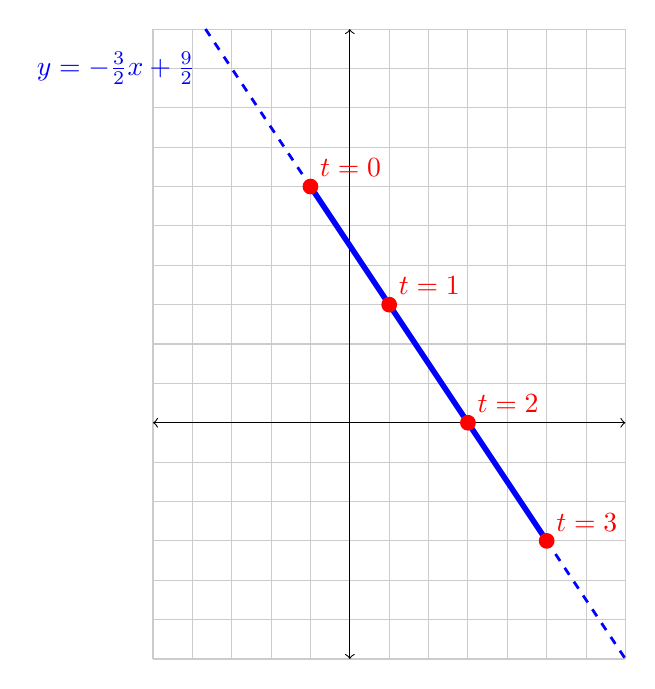
\begin{tikzpicture}[scale=0.5]
\draw[thin,gray!40] (-5,-6) grid (7,10);
  \draw[<->] (-5,0)--(7,0);
  \draw[<->] (0,-6)--(0,10);
  
\draw[line width=2pt,blue](-1,6)--(5,-3) ;

\draw[line width=1pt,blue, dashed](-11/3,10)node[below=5mm, left=0mm]{$y=-\frac{3}{2}x+\frac{9}{2}$}--(7,-6) ;

\fill[red] (-1,6) node[above right]{$t=0$} circle (0.2cm);
\fill[red] (1,3) node[above right]{$t=1$} circle (0.2cm);
\fill[red] (3,0) node[above right]{$t=2$} circle (0.2cm);
\fill[red] (5,-3) node[above right]{$t=3$} circle (0.2cm);
 \end{tikzpicture}
\end{image}

If we do not restrict $t$ to values between 0 and 3, we can get every point on the line $y=-\frac{3}{2}x+\frac{9}{2}$.  
\end{initprob}

Equations such as
\begin{align*}
x&=2t-1\\
y&=-3t+6
\end{align*}
are called \dfn{parametric equations}, and $t$ is called a \dfn{parameter}.

When given an equation of the form $y=mx+b$, we recognize it as an equation whose graph is a line and we don't need to make a table of values to sketch the graph of the equation.  We should be able to do the same for parametric equations of lines.  In the next Exploration Problem we will examine our equations carefully to see if we can discern any patterns that would help us plot the line without making a table of values.  


\begin{initprob}\label{init:paramline2dpart3}
Let's return to parametric equations from the previous problem.
\begin{align*}
x&=2t-1\\
y&=-3t+6
\end{align*}

Consider the table of values we constructed in Exploration Problem \ref{init:paramline2d}.
$$\begin{array}{|c|c|c|}  
 \hline t& x & y\\ 
 \hline 0 & -1 & 6\\ 
 \hline 1 & 1 & 3 \\
 \hline 2 & 3& 0\\
 \hline 3 & 5& -3\\
 \hline
 \end{array}$$

Observe that every time $t$ increases by $1$, $x$ increases by $2$ and $y$ decreases by $3$.  An increase by $2$ in the $x$-coordinate combined with a decrease of $3$ in the $y$-coordinate corresponds to the coefficients $2$ and $-3$ of $t$ in the parametric equations.  Our findings are in agreement with the fact that the slope of the line is $-\frac{2}{3}$.  

When only two coefficients are involved, it is convenient to use the ratio of the two coefficients, $m=\frac{\text{rise}}{\text{run}}$, but thinking ahead to higher dimensions (and more coordinates given by parametric equations), we need to find another way to communicate the same information.  

We will capture the ``rise" and ``run" aspect of the line by using vector $\vec{v}=\begin{bmatrix}2\\-3\end{bmatrix}$. Sketching $\vec{v}$ together with the line, we find that the vector is parallel to the line.  

 \begin{image}[2.8in]
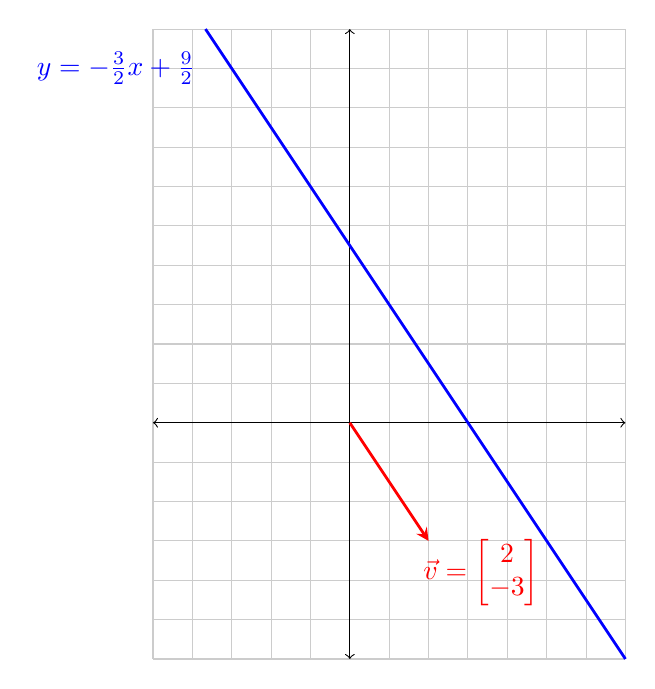
\begin{tikzpicture}[scale=0.5]
\draw[thin,gray!40] (-5,-6) grid (7,10);
  \draw[<->] (-5,0)--(7,0);
  \draw[<->] (0,-6)--(0,10);
  
\draw[line width=1pt,blue](-11/3,10)node[below=5mm, left=0mm]{$y=-\frac{3}{2}x+\frac{9}{2}$}--(7,-6) ;

\draw[line width=1pt,red, -stealth](0,0)--(2,-3)node[below=0.4cm, right=-0.2cm]{$\vec{v}=\begin{bmatrix}2\\-3\end{bmatrix}$} ;

 \end{tikzpicture}
\end{image}

Vector $\vec{v}$ is called a \dfn{direction vector}.  Observe that the components of $\vec{v}$ are the coefficients of $t$ in the parametric equations.
\begin{align*}
x&={\color{red}2}t-1\\
y&={\color{red}-3}t+6
\end{align*}

Next, let's turn our attention to constants $-1$ and $6$.  They are the values of $x$ and $y$ when $t=0$, and correspond to the point $(-1, 6)$.  

Recall that in Exploration Problem \ref{init:paramline2d} we said that the given parametric equations describe the position of a ladybug crawling in the coordinate plane.  If we are concerned with the position of the ladybug at time $t$, the point $(-1, 6)$ is very important - this is where the bug is located when $t=0$.  But, if we are using parametric equations simply to describe the line $y=-\frac{3}{2}x+\frac{9}{2}$, without regard for when the bug is located at each point, then the point $(-1, 6)$ is not any more special than any other point on the line.  In fact, we can use any other point on this line to find another set of parametric equations that describe the same line.  In Practice Problem \ref{prob:paramnotunique} you will be asked to show that equations
\begin{align*}
x&=2t+1\\
y&=-3t+3
\end{align*}
describe the same line.  Thus, parametric representations are not unique.
\end{initprob}

We can generalize our observations in Exploration Problem \ref{init:paramline2dpart3} as follows.

\begin{formula}\label{form:paramline2d}
Let $\vec{v}=\begin{bmatrix}a\\b\end{bmatrix}$ be a direction vector for line $l$, and let $(x_0, y_0)$ be an arbitrary point on $l$.  Then the following parametric equations describe $l$:
\begin{align*}
x&=at+x_0\\
y&=bt+y_0
\end{align*}
\end{formula}

\begin{example}
Find parametric equations for line $l$ if $l$ contains the point $(2, -5)$ and is parallel to line $k$ with parametric equations
\begin{align*}
x&=3t+4\\
y&=-8t+1
\end{align*}
\begin{explanation}
To find a set of parametric equations for $l$, we need a point on $l$ and a direction vector.  Point $(2, -5)$ is on $l$.  Line $l$ is parallel to $k$, so we can use $\begin{bmatrix}3\\-8\end{bmatrix}$, a direction vector for $k$, as a direction vector for $l$.   This gives us the following parametric equations for $l$:
\begin{align*}
x&=3t+2\\
y&=-8t-5
\end{align*}
\end{explanation}
\end{example}

\section*{Parametric Lines in $\RR^3$}

\begin{initprob}\label{init:paramline3d}
Consider the following set of parametric equations
\begin{align*}
x&=4t+1\\
y&=8t-3\\
z&=5t+1
\end{align*}
We will begin by making a table of values.
$$\begin{array}{|c|c|c|c|}  
 \hline t& x & y & z\\ 
 \hline -1 & -3 & -11 & -4\\ 
 \hline 0 & 1 & -3 & 1 \\
 \hline 1 & 5& 5 & 6\\
 \hline 2 & 9& 13 & 11\\
 \hline
 \end{array}$$

Observe that every time $t$ increases by $1$, $x$ increases by $4$, $y$ increases by $8$, and $z$ increases by $5$.  The pattern ``out $4$, over $8$, up $5$" is illustrated in the diagram.  


\begin{image}[4in]
\tdplotsetmaincoords{70}{130}
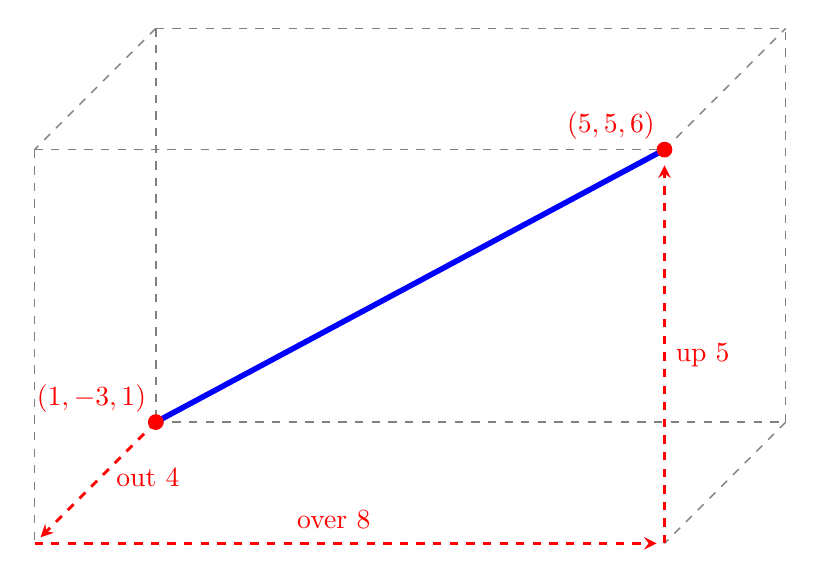
\begin{tikzpicture}
	%\draw[->](-3,0,0)--(5,0,0) node[below left]{$y$};
    %\draw[->](0,-3,0)--(0,5,0) node[below left]{$z$};
    %\draw[->](0,0,-3)--(0,0,5) node[below left]{$x$};
   
    \draw[line width=2pt,blue](-3,1,1)--(5,6,5);
    
    \draw[line width=0.5pt, dashed, gray](-3,1,1)--(5,1,1);
    \draw[line width=0.5pt, dashed, gray](5,1,1)--(5,1,5);
    \draw[line width=0.5pt, dashed, gray](5,1,1)--(5,6,1);
    \draw[line width=0.5pt, dashed, gray](5,6,5)--(5,6,1);
    \draw[line width=0.5pt, dashed, gray](-3,6,1)--(5,6,1);
    \draw[line width=0.5pt, dashed, gray](-3,6,1)--(-3,6,5);
    \draw[line width=0.5pt, dashed, gray](-3,6,1)--(-3,1,1);
    \draw[line width=0.5pt, dashed, gray](-3,6,5)--(-3,1,5);
    \draw[line width=0.5pt, dashed, gray](-3,6,5)--(5,6,5);
    
    
    \draw[line width=1pt,red, dashed, -stealth](5,1,5)--(5,5.8,5);
    \draw[line width=1pt,red, dashed, -stealth](-3,1,5)--(4.9,1,5);
     \draw[line width=1pt,red, dashed,-stealth](-3,1,1)--(-3,1,4.8);
     
     %\draw[line width=0.5pt,blue](-3,1,1)--(5,1,5);
    
    \fill[red] (-3,1,1) node[above left]{$(1,-3,1)$} circle (0.1cm); 
    \fill[red] (5,6,5) node[above left]{$(5,5,6)$} circle (0.1cm);
    
    \node[red] at (0.8, 1.3, 5)   {over $8$};
    \node[red] at (-2.1, 1.3, 3.6)   {out $4$};
    \node[red] at (5.1, 3, 4)   {up $5$};
    
\end{tikzpicture}
\end{image}

Combining numbers $4, 8, 5$ into one ratio, like we did with ``rise" over ``run," is not possible, so we use a direction vector $\vec{v}=\begin{bmatrix}4\\8\\5\end{bmatrix}$ to represent the direction of the line.  Note that the components of  $\vec{v}$ are the same as the coefficients of $t$ in the parametric equations.  

\begin{align*}
x&={\color{red}4}t+1\\
y&={\color{red}8}t-3\\
z&={\color{red}5}t+1
\end{align*}

Also, observe that the constants $1, -3, 1$ correspond to the coordinates of the point on the line for which $t=0$.

\begin{align*}
x&=4t+{\color{red}1}\\
y&=8t+({\color{red}-3})\\
z&=5t+{\color{red}1}
\end{align*}
As before, the point $(1, -3, 1)$ may be replaced with any other point on the line to produce a different set of parametric equations describing the same line.
\end{initprob}

We can generalize our observations in Exploration Problem \ref{init:paramline3d} as follows.

\begin{formula}\label{form:paramline3d}
Let $\vec{v}=\begin{bmatrix}a\\b\\c\end{bmatrix}$ be a direction vector for line $l$, and let $(x_0, y_0, z_0)$ be an arbitrary point on $l$.  Then the following parametric equations describe $l$:
\begin{align*}
x&=at+x_0\\
y&=bt+y_0\\
z&=ct+z_0
\end{align*}
\end{formula}

\begin{example}\label{ex:paramline3d}
Find a set of parametric equations for a line in $\RR^3$ that passes through $(1, -2, 4)$ and $(-3, 1, 1)$.
\begin{explanation}
We need a point and a direction vector.  To find the direction vector we will use the ``head-tail" formula (Formula \ref{form:headminustailrn}) to find the vector whose tail is at $(1, -2, 4)$ and whose head is at $(-3, 1, 1)$.  The direction vector is
$$\begin{bmatrix}-3-1\\1-(-2)\\1-4\end{bmatrix}=\begin{bmatrix}-4\\3\\-3\end{bmatrix}$$
For our point, we can pick either of the two given points.  The equations will differ depending on the point we pick, but they will describe the same line.  Remember, parametric representations are not unique!  If we choose $(1, -2, 4)$ for our point we get the following set of parametric equations:
\begin{align*}
x&=-4t+1\\
y&=3t-2\\
z&=-3t+4
\end{align*}
\end{explanation}
\end{example}

\section*{Parametric Lines in $\RR^n$}
After working with parametric equations of lines in $\RR^2$ and $\RR^3$, it should be easy to surmise what parametric equations of lines look like for lines in $\RR^n$.
\begin{formula}\label{form:paramlinend}
Let $\vec{v}=\begin{bmatrix}v_1\\v_2\\\vdots\\v_n\end{bmatrix}$ be a direction vector for line $l$ in $\RR^n$, and let $(a_1, a_2,\ldots , a_n)$ be an arbitrary point on $l$.  Then the following parametric equations describe $l$:
\begin{align*}
x_1&=v_1t+a_1\\
x_2&=v_2t+a_2\\
&\quad\vdots\\
x_n&=v_nt+a_n
\end{align*}
\end{formula}


\section*{Practice Problems}

\begin{problem}\label{prob:paramnotunique}
In Exploration Problems \ref{init:paramline2d}, \ref{init:paramline2dpart2} and \ref{init:paramline2dpart3} you encountered a set of parametric equations
\begin{align*}
x&=2t-1\\
y&=-3t+6
\end{align*}
Show that the following parametric equations describe the same line.
\begin{align*}
x&=2t+1\\
y&=-3t+3
\end{align*}
\end{problem}

\begin{problem}
Find two different parametric representations for a line with slope $3$ and $y$-intercept $(0, -4)$.
\end{problem}

\begin{problem}
Find a parametric representation for line $l$ passing through $(4, -2, 5)$ if line $l$ has a direction vector parallel to that of the line with parametric equations 
\begin{align*}
x&=t-4\\
y&=3t\\
z&=7t+1
\end{align*}
\end{problem}

\begin{problem} Find a direction vector for a line that passes through $(-2, 1, -3)$ and $(5, -7, 9)$.  Is the direction vector you found unique?
\end{problem}

\begin{problem}
Find a direction vector for a line given by parametric equations
\begin{align*}
x_1&=t+3\\
x_2&=t-4\\
x_3&=3t\\
x_4&=7t+1
\end{align*}
\end{problem}

\begin{problem}
What can you say about two lines in $\RR^2$ if the dot product of their direction vectors is $0$?
\end{problem}

\end{document} 